% !TEX root = main.tex
\chapter{Demonstration}\label{sec:demonstration}
To better explain how ReviewerNet works and supports the reviewer selection process, this section presents an example user scenario. We introduce Robert, a fictitious academic researcher. Robert is in the IPC of a conference in the field of Computer Graphics; he is the primary reviewer for a paper, and he is in charge of finding three additional reviewers, plus alternative reviewers in case of decline. 
Below we describe Robert's interaction with ReviewerNet
\subsection*{Starting ReviewerNet}

Robert is in charge of finding reviewers for a paper about polycube maps, authored by Marco Tarini and Daniele Panozzo. In the Control Panel area, he inputs their names in the \emph{Submitting Researchers} field, also with the help of a drop-down menu. The authors are now shown in the Researcher Timeline and the Reviewer Network, marked as purple. 
\subsection*{Building the Paper Network} 
%\label{sec:demoPN}
The first step is to build the Paper Network (Figure \ref{fig:keypapers}), that is, a set of key papers which are relevant to the submission topic. Later on, Robert will chose his reviewers among the authors of those key papers. Robert  thinks of a first pair of documents about polycube maps, which serve as seeds for building the network (\emph{PolyCube-Maps}, 2004; \emph{Polycube simplification for coarse layouts of surfaces and volumes}, 2016.  %\emph{A divide-and-conquer approach for automatic polycube maps construction}, 2009; \emph{$L_1$-based construction of polycube maps from complex shapes}, 2014). 
He inputs their titles in the \emph{Key papers} field. His knowledge of the domain helps him in this initial step, though he can also take advantage of title- and author- based suggestions, which are shown in a drop-down menu, listed by publication year. Also, the list of references in the submitted paper or in previously identified seed papers can provide a convenient strategy to initialize the network. Robert copies (a subset of) citations in the \emph{Import from bibliography} window, and the system returns the list of matching papers in the dataset (Figure \ref{fig:keypapers_2}). Robert can now approve or discard the suggestions. He ends up adding three more papers (\emph{A divide-and-conquer approach for automatic polycube maps construction}, 2009; \emph{$L_1$-based construction of polycube maps from complex shapes}, 2014; \emph{All-hex mesh generation via volumetric polycube deformation}, 2011). 
The five papers are now included in the Paper Network, along with their in- and out-citations. 
 
While Robert builds his Paper Network, ReviewerNet automatically adds the authors of selected papers in the Researcher Timeline and the Researcher Network, as candidate reviewers.

Robert can now expand the Paper Network, to discover additional documents and therefore additional candidate reviewers. Papers which cite (are cited) by a single key paper are displayed along a common line, and clustered by year. Papers which cite (are cited) by more than one key paper are good candidates for being added, therefore, they are positioned in-between key paper lines, so that they can be easily identified as interesting nodes. With a double click, Robert selects  papers he deems relevant to polycube maps. The Paper Network then updates with the in- and out-citations of the selected papers, so that Robert can further explore the literature. Robert navigates the network, and decides to reduce its size by deselecting a paper he realizes he is no longer interested in, because its citations suggest it addresses a different topic than the submission. %Selected papers are marked with a blue contour circle, both in the Paper Network and the Researcher Network. 
Robert continues until he feels the selected papers and their citations offer a good coverage of the literature about the topic at hand. Robert checks the paper details, including the link to the respective DBLP page, shown in the bottom right corner of the interface. A quick keyword search with \emph{polycube maps} in the \emph{Key papers} field let him notice that there is an important paper he was missing (\emph{Interactive applications for sketch-based editable polycube maps, 2016}); the paper can be easily told apart from papers already in the network, thanks to visual cues in the drop-down menu. Finally, the selection of 6 papers produces a list of 23 candidate reviewers. 


\begin{figure*}[!pt]
    \centering
    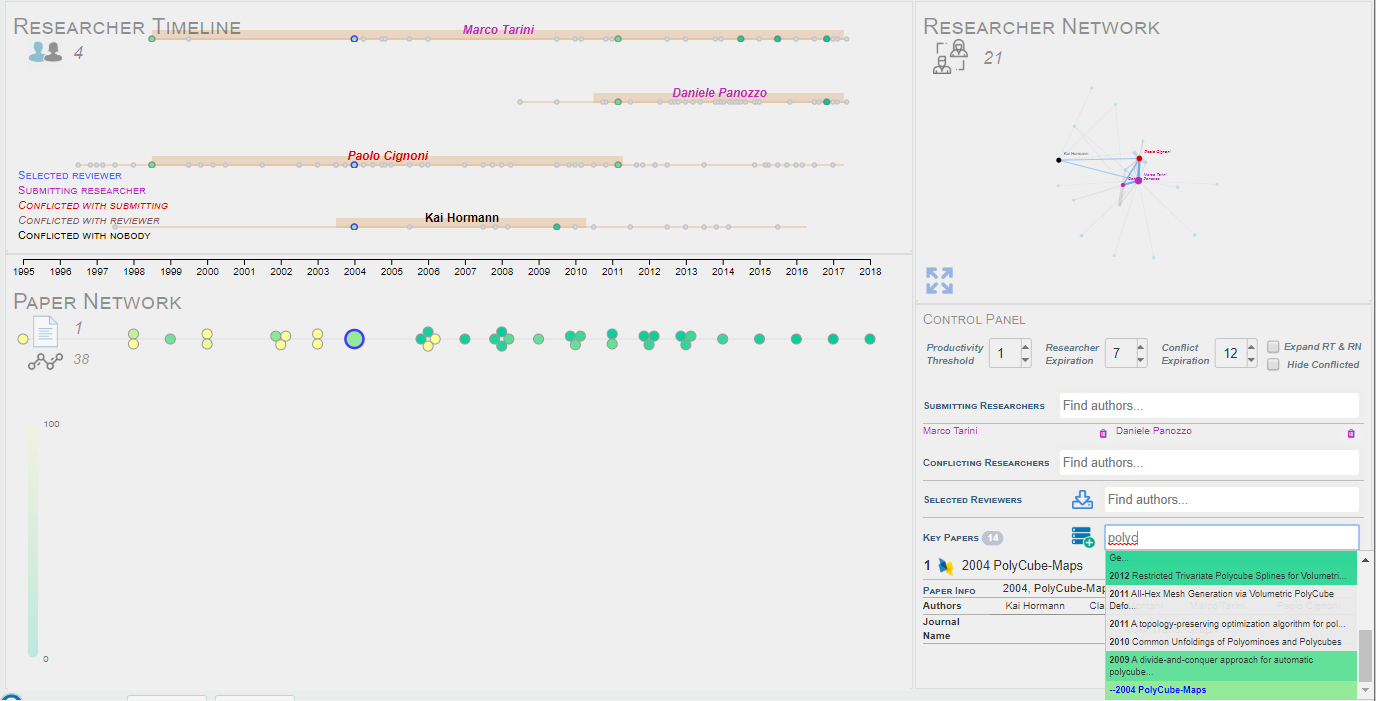
\includegraphics[width=\textwidth]{fig/insertion_manual.png}		
    \caption{When the user inputs the seed papers (bottom right), ReviewerNet starts building the Paper Network (bottom left), the Researcher Timeline (top left), and the Researcher Network (top right). The dots representing papers in the Paper Network and the Researcher Timeline are coloured according {either to their citation count -- from green (few citations) to yellow (many citations) -- or to the venue they were published in}. Grey dots in the Researcher Timeline are papers in the reference database, but not included in the current Paper Network. Selected papers are circled in blue.}%When hovering over an entity representing a paper, the authors of that paper are highlighted in the other views.}
    \label{fig:keypapers}
    \end{figure*}
    
\begin{figure*}[!p]
    \centering
    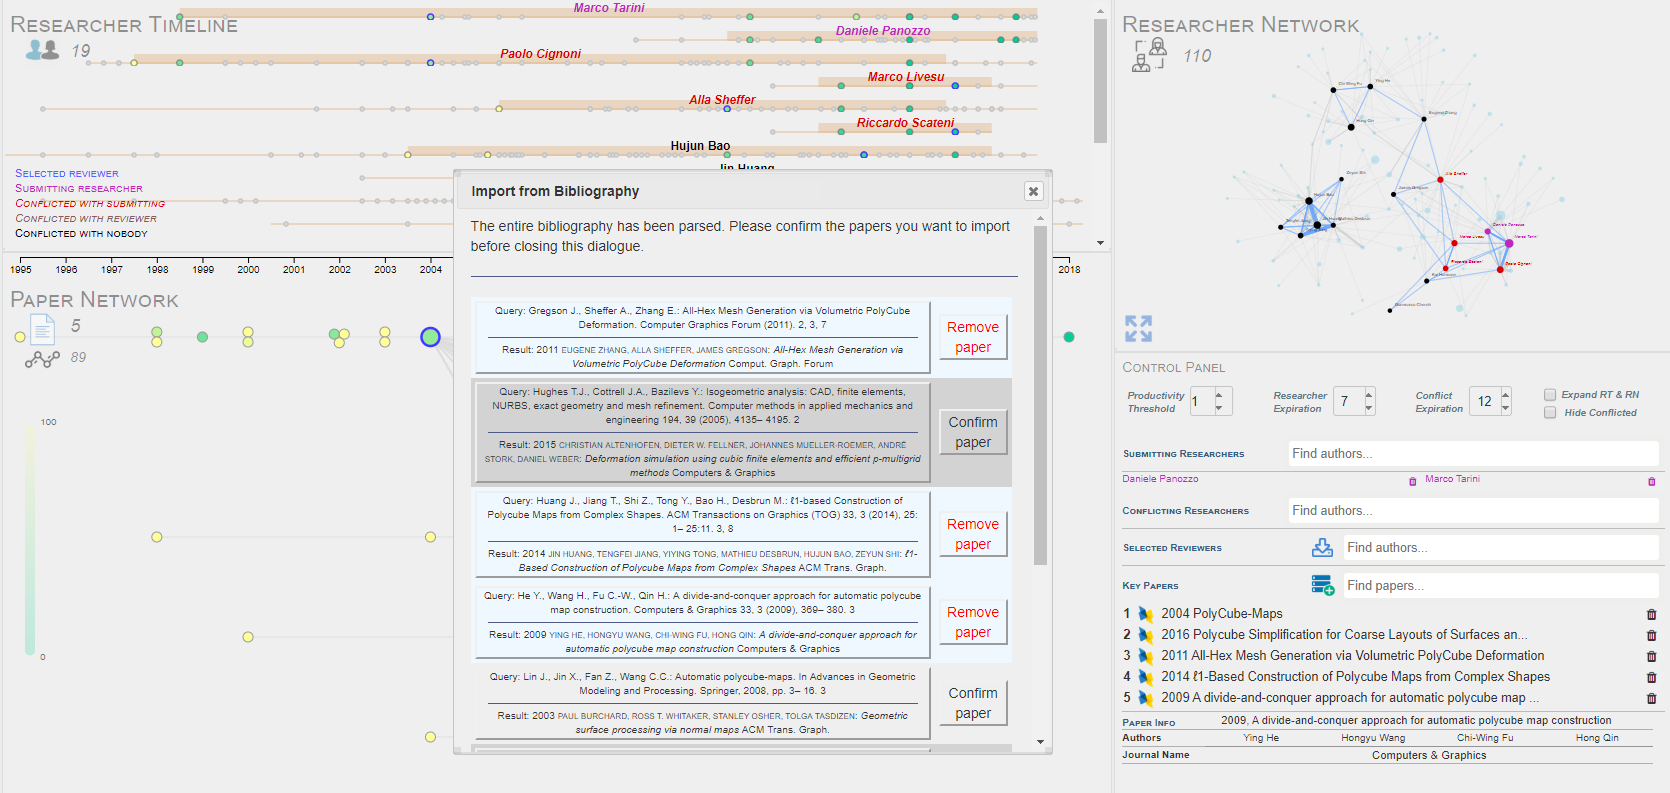
\includegraphics[width=\textwidth]{fig/insertion_biblio.png}		
    \caption{The seed papers can be imported from the bibliography of a paper. The user can copy and paste the references, which are parsed by the system; matching titles in the dataset are returned and submitted to the user for either approval or rejection.}%When hovering over an entity representing a paper, the authors of that paper are highlighted in the other views.}
    \label{fig:keypapers_2}
\end{figure*}
    


\subsection*{Exploring the Researcher Timeline and the Researcher Network} 
 
Robert now explores the Researcher Timeline to assess the suitability of candidate reviewers. In the Researcher Timeline, researchers are represented as horizontal lines, spanning their academic career. Robert checks the expertise of candidate reviewers by looking at their stage of career, and production over years. Since each view is linked to the other views, Robert checks topic coverage by looking at who published what, by hovering the mouse over papers to highlight their authors in all the views (Figure \ref{fig:overpaper}). With a mouse click on a researcher, ReviewerNet highlights both his/her co-authors and papers (Figure \ref{fig:authorclick}).
While looking for candidate reviewers, Robert can always checks conflicts of interests, thanks to colours and font style (Figure \ref{fig:selected}). 

The visualization also helps Robert analysing the network of collaborators of candidate reviewers. This is fundamental to find sets of independent, well distributed reviewers. Robert can navigate the Researcher Network, a graph visualization of co-authorship relations among the candidate reviewers and their collaborators in the dataset. He switches to full-screen mode, then pans and zooms and uses the different handlers available to discover conflicts-of-interest of different degrees, as well as to identify network cliques that represent communities of collaborators. He founds out that there are three distinct groups of collaborators dealing with the topic at hand (Figure \ref{fig:communities}).

%\begin{figure}[!pt]
%\centering
%\includegraphics[width=0.4\textwidth]{fig/highlighting_coauthor.png}
%\caption{.}%When hovering over an entity representing a paper, the authors of that paper are highlighted in the other views.}
%\label{fig:common}
%\end{figure}

\paragraph*{Selecting reviewers} 

Once Robert identifies one or more candidate reviewers, he inputs their names in the \emph{Selected Reviewers} field (also with the help of the drop-down menu). He decides to chose Gustavo Patrow, whose expertise fits with his requirements.  The colouring of the selected reviewer switches to blue both in the Researcher Timeline and the Researcher Network, and the colouring of his co-authors switches to grey, to identify them as conflicting potential reviewers, and tell them apart from the remaining available candidates. Then, Robert selects Hujun Bao, a senior researcher, and Gianmarco  Cherchi, a younger researcher who belongs to a different community than the previous two, and has been working very recently on the subject at hand. The icon beside the reviewers name links to their respective DBLP pages, so that Robert can further check about conflicts of interest possibly deriving from the co-authorship of papers published on venues not included in the dataset.

Robert downloads his list of three reviewers with a click on the download button. The list reports reviewers' names and bibliographic references to their papers (Figure \ref{fig:list}). After contacting the reviewers, Robert finds that one of them declines his invitation. Fortunately, for each reviewer selected by Robert, ReviewerNet has automatically added a list of potential alternative reviewers, in case of a negative answer by the original reviewer. Alternative reviewers are chosen from the candidate ones, so that they only conflict with the declining reviewer. Robert evaluates possible substitutes, again taking advantage of ReviewerNet functionalities, and finds his best replacement. 

\begin{figure}[!pt]
\centering
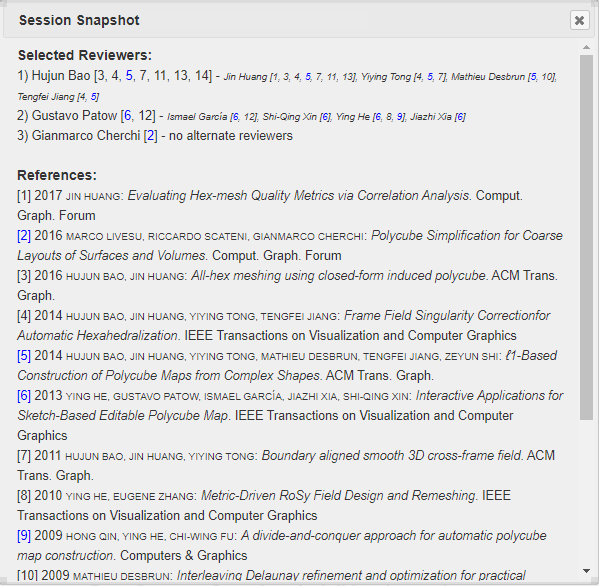
\includegraphics[width=0.8\textwidth]{fig/reviewers.png}
\caption{The list of selected reviewers, together with substitutes in case of decline, and a bibliography. A substitute reviewer is a researcher who has authored a similar set of publications and has the same conflicts as the original reviewer. The bibliography motivates the  reviewer selection, since it lists, for each selected reviewer, the papers he/she has authored.}%When hovering over an entity representing a paper, the authors of that paper are highlighted in the other views.}
\label{fig:list}
\end{figure}

 

\paragraph*{Discussion} 
This abbreviated scenario shows how ReviewerNet can support investigating the literature, learning who are the experts in a field, and exploring relationships among them. The description above necessarily simplified a typical interaction process: Robert could of course switch back and forth between different tasks; as the coherence of visual cues across different views enforces their meaningfulness, it is easy for him to switch between different views without losing focus. Robert could have also refined the Paper Network after having examined the list of candidate reviewers. He could have adjusted the size of the list by fine tuning the optional parameters. The process is iterative in nature, and the desiderata may evolve as the search proceeds. Thanks to the user-friendly interface which leaves the user control over the process, ReviewerNet enables the user to narrow down as well as widen the scope of analysis. In turn, the combined visualization of different aspects of the problem at hand well supports the decision making process.     
